\subsection*{2.3}
The assumption that a vertex in G can have a degree no higher than 4 is
necessary as there are only 4 possible "entrances" to a vertex when it is drawn
on a rectilinear form. 
\begin{figure}[!ht]
    \centering
    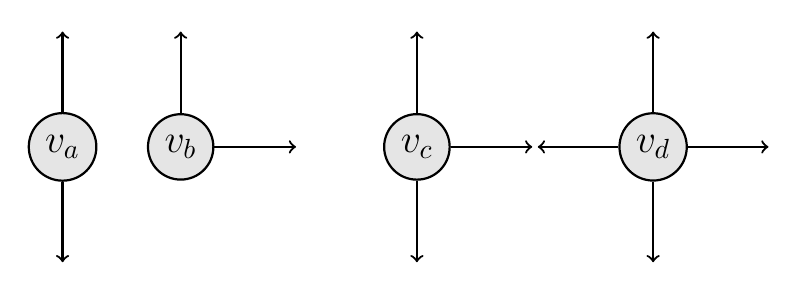
\begin{tikzpicture}[->,shorten >=1pt,auto,node distance=1.5cm,
  thick,main node/.style={circle,fill=gray!20,draw,font=\sffamily\Large\bfseries}]


  \node[main node] (2) {$v_a$};
  \coordinate[above of=2] (d5);
  \coordinate[below of=2] (d6);

  \node[main node] (3) [right of=2] {$v_b$};
  \coordinate[above of=3] (d7);
  \coordinate[right of=3] (d8);

  \node[main node] (4) [right of=d8] {$v_c$};
  \coordinate[above of=4] (d9);
  \coordinate[right of=4] (d10);
  \coordinate[below of=4] (d11);

  \node[main node] (1) [right of=d10] {$v_d$};
  \coordinate[left of=1] (d1);
  \coordinate[right of=1] (d2);
  \coordinate[above of=1] (d3);
  \coordinate[below of=1] (d4);

  \path[every node/.style={font=\sffamily\small}]
  (1)  edge [] node[above] {} (d1)
       edge [] node[above] {} (d2)
       edge [] node[above] {} (d3)
       edge [] node[above] {} (d4)

  (2)  edge [] node[above] {} (d5)
       edge [] node[above] {} (d6)

  (3)  edge [] node[above] {} (d7)
       edge [] node[above] {} (d8)

  (4)  edge [] node[above] {} (d9)
       edge [] node[above] {} (d10)
       edge [] node[above] {} (d11);
\end{tikzpicture} 

    \caption{The 4 vertex cases depending on its degree} 
    \label{fig:degree}
\end{figure}

In figure \ref{fig:degree} the possible cases for the vertices can be seen.
If v is of degree 2 and placed between boundary cycles $f_1$ and $
f_2$ there are two cases. One where there is no turn in the vertex and
one where there is a single turn. In the first case both $x_{vf_1}$ and
$x_{vf_2}$ will be zero. In the second case the turn will be an outer turn
in regards to one of the cycles and an inner turn in regards to the other.
The sum is zero in this case as well.

If v is of degree 3 and placed between boundary cycles $f_1$, $f_2$ and $f_3$
there is one case. It will be a T-cross where the vertex is flat in regards to
one of the cycles and an inner turn for the two others. The sum is then 2.
If v is of degree 4 and placed between boundary cycles $f_1$, $f_2$,
$f_3$ and $f_4$ there is one case. In this case it will be a cross in the
middle of the 4 cycles and it will form 4 inner circles. Thus the sum is 4.
There are no more cases and the form held for all of them.


